\documentclass{article}
\oddsidemargin=1cm
\usepackage[spanish]{babel}%paquete principal2
\usepackage[utf8]{inputenc}%paquete principal2
\usepackage{latexsym} % Simbolos 
\usepackage{graphicx} % Inclusion de graficos. Soporte para figura 
\usepackage{hyperref} % Soporte hipertexto
\usepackage{subfigure}
\usepackage{epsfig}
\usepackage{graphicx}
\usepackage{rotating}
\usepackage{epstopdf}
\usepackage{ctable}
\usepackage{longtable}
\usepackage{color}
\usepackage{colortbl}
\usepackage{tabularx,colortbl}
\usepackage{setspace}
\usepackage{threeparttable}
\usepackage{multirow}
\usepackage{pdflscape}
\usepackage{anysize}
%\usepackage[authoryear]{natbib}
\usepackage{breakurl}
\usepackage{url}
\usepackage{amssymb}
\usepackage{graphicx}
\usepackage[centertags]{amsmath}
\usepackage{amsthm}
\usepackage{array}
\usepackage{times}
\usepackage[left=1in, right=1in, top=1in, bottom=1in]{geometry}
\usepackage{rotating}
\usepackage{amstext}
\usepackage{pdfpages}
\usepackage{amsbsy}
\usepackage{amsopn}
\usepackage{eucal}
\usepackage{sectsty}
\usepackage{titlesec}
\usepackage[capposition=top]{floatrow}
\usepackage{pdfpages}
\usepackage{apacite}
%\usepackage[singlespacing]{setspace}
\usepackage[labelsep=period,font={bf},textfont={normalsize},labelfont={normalsize}]{caption}
%\usepackage[longnamesfirst,comma]{natbib}
%\usepackage{iadb}
\title{\textbf{Estrategia de Comunicación} \\ ''Competencia Boliviana de Posters Estadísticos ''}
\author{Fundación ARU}
\date{2018-2019 }
\begin{document} % Inicio del documento
\maketitle

\hrule
\hrule
\newpage

%%%%%%%%%%%%%%%%%%%%%%%%%%%%%%%%%%%%%%%%
\section{Introducción}

El plan de comunicación es una propuesta para el logro de los objetivos de la Competencia Boliviana de Posters Estadísticos 2018-2019 del proyecto ''Alfabetización Estadística''. Plan dirigido a captar a las personas nacidas desde el año 2000 hasta el año 2005 y personas que estudian en la universidad.\\

En el se podrá encontrar una descripción de la organización, y desarrollo de la sociabilización de la competencia llevada por primera vez en Bolivia.


\section{Objetivos}

\begin{itemize}
\item Promocionar la competencia para lograr despertar el interés en personas nacidas el año 2000 hasta el año 2005 y personas que estudian en la universidad a nivel nacional. 

\item Difundir en diversos canales de comunicación la existencia de la competencia asi como los principales requerimientos técnicos para participar en cada etapa de la competencia.
\end{itemize} 

\section{Definición de actores objetivo}

La competencia esta dirigida a personas nacidas desde el año 2000 hasta el 2005 y personas que estudian en el pregrado en las universidades públicas y privadas de toda Bolivia, asimismo las personas deben contar con el apoyo de un tutor profesional que acompañe su trabajo y les sirva de guía, en este sentido se prevee que los actores clave sean las personas antes mencionadas, tutores y entidades que al recibir toda ésta información puedan formar parte del grupo patrocinador.

\section{Implementación}

Dado los objetivos esperados, se propone la siguiente linea de implementación para el proyecto:

\begin{enumerate}
\item Presentación del proyecto\footnote{Ver anexo \ref{prog}}
\begin{itemize}
\item Audiencia esperada:
\begin{itemize}
\item Representante de la Iniciativa
\item Institución Organizadora
\item Patrocinadores
\item Personas nacidas desde el año 2000 hasta el 2005
\item Personas que estudian en la universidad
\end{itemize}
\item Fecha tentativa:
\begin{itemize}
\item 29 de Junio
\end{itemize}
\item Objetivo
\begin{itemize}
\item Presentar el proyecto
\item Presentar la convocatoria
\item Presentar a las instituciones involucradas
\item Presentar los medios disponibles para la cobertura en participación
\begin{itemize}
\item Página de la iniciativa 
\item Canal de facebook
\item Canal de twitter
\end{itemize}
\end{itemize}
\item Estrategia
\begin{itemize}
\item Internet
\end{itemize}
\end{itemize}

\item Difusión en sitio web redes sociales, dirigido al público en general 
\begin{itemize}
\item Audiencia esperada:
\begin{itemize}
\item Personas nacidas desde el año 2000 hasta el 2005
\item Personas que estudian en la universidad
\end{itemize}
\item Fecha tentativa:
\begin{itemize}
\item 29 de Junio del 2018 - 14 de Enero del 2019
\end{itemize}
\item Objetivo
\begin{itemize}
\item Mantener informado al público del proyecto
\item Presentar fuentes de información disponibles
\item Proponer tutoriales de manejo de información
\begin{itemize}
\item Página de la iniciativa 
\item Canal de facebook
\item Canal de twitter
\item Programación de talleres de apoyo a participantes
\end{itemize}
\end{itemize}
\item Herramienta de apoyo
\begin{itemize}
\item Internet
\end{itemize}
\end{itemize}

\item Diseño de esquema de funcionamiento del proyecto
\begin{itemize}
\item Audiencia esperada:
\begin{itemize}
\item Comite organizador
\item Instituciones Auspiciadoras
\end{itemize}
\item Fecha tentativa:
\begin{itemize}
\item 22 de Febrero del 2018 - Mayo 2018
\end{itemize}
\item Objetivo
\begin{itemize}
\item Delimitar tareas
\begin{itemize}
\item Recepción de poster físicos
\item Distribución de afiches de la convocatoria
\item Repositorio de bases de datos disponibles
\item Preparación de materiales de comunicación
\item Cronograma de actividades
\item Propuesta económica
\end{itemize}
\end{itemize}
\item Estrategia
\begin{itemize}
\item Reuniones y acuerdos de cooperación
\end{itemize}
\end{itemize}

\item Spot, afiches publicitarios* 
\begin{itemize}
\item Audiencia esperada:
\begin{itemize}
\item Personas nacidas desde el año 2000 hasta el 2005
\item Personas que estudian en la universidad
\item Profesores y docentes
\end{itemize}
\item Fecha tentativa:
\begin{itemize}
\item 29 de Junio del 2018 - Agosto del 2018
\end{itemize}
\item Objetivo
\begin{itemize}
\item Crear un corto de video que transmita la convocatoria y publicarlo en:
\item Tener un medio corto, que de a conocer el concurso
\begin{itemize}
\item Página de la iniciativa 
\item Canal de facebook
\item Canal de twitter
\end{itemize}
\end{itemize}
\item Estrategia
\begin{itemize}
\item Internet
\end{itemize}
\end{itemize}
* ver anexos

\item Talleres de sociabilización** 
\begin{itemize}
\item Audiencia esperada:
\begin{itemize}
\item Personas nacidas desde el año 2000 hasta el 2005
\item Personas que estudian en la universidad
\item Profesores y docentes
\end{itemize}
\item Fecha tentativa:
\begin{itemize}
\item 29 de Junio del 2018 - Agosto del 2018
\end{itemize}
\item Objetivo
\begin{itemize}
\item Motivar a la audiencia a participar de la convocatoria
\end{itemize}
\item Estrategia
\begin{itemize}
\item Personal recorriendo puntos centrales
\end{itemize}
\end{itemize}

**Participación en eventos para publicitar el proyecto

\item Canales de Comunicación: ARU - Patrocinadores
\begin{itemize}
\item Actores principales:
\begin{itemize}
\item Entidad organizadora
\item Instituciones patrocinadoras
\end{itemize}
\item Fecha tentativa:
\begin{itemize}
\item 29 de Junio del 2018 - Enero 2019
\end{itemize}
\item Objetivo
\begin{itemize}
\item Publicitar la convocatoria
\item Mantener lazos de comunicación con los auspiciadores (actividades e invitaciones)
\item Coordinar instrumentos y materiales para el concurso
\end{itemize}
\item Vías de comunicación
\begin{itemize}
\item Internet (correo electrónico, página en internet, medios sociales)
\item Teléfono celular, teléfono fijo
\end{itemize}
\end{itemize}

\item Materiales publicitarios
\begin{itemize}
\item Audiencia esperada:
\begin{itemize}
\item Personas nacidas desde el año 2000 hasta el 2005
\item Personas que estudian en la universidad
\end{itemize}
\item Fecha tentativa:
\begin{itemize}
\item 29 de Junio del 2018 - Agosto del 2018
\end{itemize}
\item Objetivo
\begin{itemize}
\item Motivar la participación de las personas
\item Informar a la audiencia de la convocatoria
\item Publicar posters informativos
\item Publicar folletos de información y convocatoria
\end{itemize}
\item Personas involucradas
\begin{itemize}
\item Personal de la entidad organizadora 
\item Instituciones patrocinadoras
\end{itemize}
\end{itemize}


\item Cierre de clausura
\begin{itemize}
\item Audiencia esperada:
\begin{itemize}
\item Representante de la Iniciativa
\item Institución Organizadora
\item Patrocinadores
\item Personas nacidas desde el año 2000 hasta el 2005
\item Personas que estudian en la universidad
\end{itemize}
\item Fecha tentativa:
\begin{itemize}
\item 29 de Marzo del 2019
\end{itemize}
\item Objetivo
\begin{itemize}
\item Presentar a las instituciones involucradas
\item Dar ha conocer el alcance de la iniciativa
\item Presentar a los ganadores de la convocatoria
\item Premiar a los ganadores de la competencia
\end{itemize}
\item Estrategia
\begin{itemize}
\item Internet, correo electrónico
\end{itemize}
\end{itemize}
\end{enumerate}


\section{Presupuesto}

El cuadro \ref{ppp} presenta el presupuesto planificado para la competencia, este presupuesto se enfoca en los gastos para la premiación y el material de difusión. 

\begin{table}[htbp]
  \centering
  \caption{Presupuesto}
  \scalebox{0.7}{
    \begin{tabular}{ll|r}
    \toprule
    \multicolumn{1}{c|}{\textbf{Actividad}} & \multicolumn{1}{c|}{\textbf{Detalle}} & \multicolumn{1}{c}{\textbf{Monto en Sus.}} \\
    \midrule
    \midrule
    \multicolumn{1}{l|}{\multirow{5}[2]{*}{Presentación del proyecto}} & \textbf{1. Evento de lanzamiento} & \multicolumn{1}{c}{\multirow{5}[2]{*}{}} \\
    \multicolumn{1}{l|}{} & 1.1. Lanzamiento de la competencia en acto público &  \\
    \multicolumn{1}{l|}{} & 1.2. Provisión de material de apoyo &  \\
    \multicolumn{1}{l|}{} & 1.3. Mensajería  &  \\
    \midrule
    \multicolumn{1}{l|}{\multirow{4}[2]{*}{Diseño e impresión de materiales}} & \textbf{2. Afiches de difusión (300 unidades)} & \multicolumn{1}{c}{\multirow{4}[2]{*}{500}} \\
    \multicolumn{1}{l|}{} & 2.1. Diseño de afiches &  \\
    \multicolumn{1}{l|}{} & 2.2. Impresión de afiches &  \\
    \midrule
    \multicolumn{1}{l|}{\multirow{3}[2]{*}{Difusión}} & \textbf{3. Material de promoción} & \multicolumn{1}{c}{\multirow{3}[2]{*}{}} \\
    \multicolumn{1}{l|}{} & 3.1. Sitio web &  \\
    \multicolumn{1}{l|}{} & 3.2. Redes sociales &  \\
    \multicolumn{1}{l|}{} & 3.3. Spot publicitario &  \\
    \midrule
    \multicolumn{1}{l|}{\multirow{3}[2]{*}{Premiación y clausura}} & \textbf{5. Premiación} & \multicolumn{1}{c}{\multirow{3}[2]{*}{1000}} \\
    \multicolumn{1}{l|}{} & 5.1. Anuncio de los ganadores en las categorías &  \\
    \multicolumn{1}{l|}{} & 5.2. Premiación de grupos ganadores &  \\
    \midrule
    \multicolumn{2}{l|}{\textbf{Total}} & 1500 \\
    \bottomrule
    \end{tabular}}%
  \label{ppp}%
\end{table}%


% Table generated by Excel2LaTeX from sheet 'Hoja1'
\begin{table}[htbp]
  \centering
    \scalebox{0.65}{
  \caption{Presupuesto para ''Paquete Estudiantil'' - Premio}
    \begin{tabular}{|cccc|r|r|r}
    \toprule
    \multicolumn{1}{|l|}{\textbf{Nro}} & \multicolumn{1}{l|}{\textbf{Cantidad}} & \multicolumn{1}{l|}{\textbf{Descripción del producto}} & \multicolumn{1}{l|}{\textbf{Precio}} & \multicolumn{1}{l|}{\textbf{Total (bs)}} & \multicolumn{1}{l|}{\textbf{Total(Sus) 6,86}} & \multicolumn{1}{l|}{\textbf{Detalle}} \\
    \midrule
    \multicolumn{1}{|r|}{1} & \multicolumn{1}{c|}{15} & \multicolumn{1}{l|}{Cartapacio - 3 anilla carta c/visor 200 h, 29 cm Blanco} & \multicolumn{1}{r|}{38} & 570   & 83,09 & \multicolumn{1}{l|}{Premio} \\
    \midrule
    \multicolumn{1}{|r|}{2} & \multicolumn{1}{c|}{45} & \multicolumn{1}{l|}{Papel bond carta - 500 h 75 gr. Blanco} & \multicolumn{1}{r|}{37} & 1665  & 242,71 & \multicolumn{1}{l|}{Premio} \\
    \midrule
    \multicolumn{1}{|r|}{3} & \multicolumn{1}{c|}{45} & \multicolumn{1}{l|}{Bolígrafo - azul, Pointec Transparente} & \multicolumn{1}{r|}{2,1} & 94,5  & 13,78 & \multicolumn{1}{l|}{Premio} \\
    \midrule
    \multicolumn{1}{|r|}{4} & \multicolumn{1}{c|}{45} & \multicolumn{1}{l|}{Bolígrafo - rojo, Pointec Transparente} & \multicolumn{1}{r|}{2,1} & 94,5  & 13,78 & \multicolumn{1}{l|}{Premio} \\
    \midrule
    \multicolumn{1}{|r|}{5} & \multicolumn{1}{c|}{45} & \multicolumn{1}{l|}{Bolígrafo - negro, Pointec Transparente} & \multicolumn{1}{r|}{2,1} & 94,5  & 13,78 & \multicolumn{1}{l|}{Premio} \\
    \midrule
    \multicolumn{1}{|r|}{6} & \multicolumn{1}{c|}{30} & \multicolumn{1}{l|}{Pegamento - barra 40 gr stick} & \multicolumn{1}{r|}{22,5} & 675   & 98,40 & \multicolumn{1}{l|}{Premio} \\
    \midrule
    \multicolumn{1}{|r|}{7} & \multicolumn{1}{c|}{15} & \multicolumn{1}{l|}{Engrampadora mediana - 12 cm metal } & \multicolumn{1}{r|}{35,9} & 538,5 & 78,50 & \multicolumn{1}{l|}{Premio} \\
    \midrule
    \multicolumn{1}{|r|}{8} & \multicolumn{1}{c|}{30} & \multicolumn{1}{l|}{Perforadora pequeña - Ne c/Plomo} & \multicolumn{1}{r|}{21} & 630   & 91,84 & \multicolumn{1}{l|}{Premio} \\
    \midrule
    \multicolumn{1}{|r|}{9} & \multicolumn{1}{c|}{30} & \multicolumn{1}{l|}{Tijera grande} & \multicolumn{1}{r|}{15} & 450   & 65,60 & \multicolumn{1}{l|}{Premio} \\
    \midrule
    \multicolumn{1}{|r|}{10} & \multicolumn{1}{c|}{15} & \multicolumn{1}{l|}{Portamina - metal} & \multicolumn{1}{r|}{14,8} & 222   & 32,36 & \multicolumn{1}{l|}{Premio} \\
    \midrule
    \multicolumn{1}{|r|}{11} & \multicolumn{1}{c|}{15} & \multicolumn{1}{l|}{Minas negras} & \multicolumn{1}{r|}{3,3} & 49,5  & 7,22  & \multicolumn{1}{l|}{Premio} \\
    \midrule
    \multicolumn{1}{|r|}{12} & \multicolumn{1}{c|}{15} & \multicolumn{1}{l|}{Hojas carta 300 hojas a color} & \multicolumn{1}{r|}{75} & 1125  & 163,99 & \multicolumn{1}{l|}{Premio} \\
    \midrule
    \multicolumn{1}{|r|}{13} & \multicolumn{1}{c|}{45} & \multicolumn{1}{l|}{Resaltador grueso amarillo} & \multicolumn{1}{r|}{4,2} & 189   & 27,55 & \multicolumn{1}{l|}{Premio} \\
    \midrule
    \multicolumn{1}{|r|}{14} & \multicolumn{1}{c|}{45} & \multicolumn{1}{l|}{Bloc adhesivo mediano - 76*76 fluorescente amarillo} & \multicolumn{1}{r|}{6,8} & 306   & 44,61 & \multicolumn{1}{l|}{Premio} \\
    \midrule
    \multicolumn{1}{|r|}{15} & \multicolumn{1}{c|}{16} & \multicolumn{1}{l|}{Hojas Adhesivas para logos} & \multicolumn{1}{r|}{5} & 80    & 11,66 & \multicolumn{1}{l|}{Premio} \\
    \midrule
    \multicolumn{1}{|r|}{16} & \multicolumn{1}{c|}{1000} & \multicolumn{1}{l|}{Afiches} & \multicolumn{1}{r|}{3,5} & 3500  & 510,20 & \multicolumn{1}{l|}{Publicidad} \\
    \midrule
    \multicolumn{4}{|c|}{\textbf{Total}} & \textbf{10283,5} & \textbf{1500.00} &  \\
\cmidrule{1-6}    \end{tabular}}%
  \label{tab:addlabel}%
\end{table}%



\section{Esquema de Organización}

El equipo de trabajo necesario para el buen desarrollo delas actividades involucradas con la Competencia Boliviana de Posters estadísticos es el siguiente: 

\begin{itemize}
\item Representante de la iniciativa: Alvaro Chirino.  
\item Institución Organizadora: Fundación ARU.
\item Responsable de medios de difusión:  Fundación ARU y patrocinadores. 
\item Responsable del manejo de redes sociales: Fundación ARU.
\item Responsable de publicación de carteles y afiches de Información: INE.
\item Recepción de poster físicos: INE.
\item Recepción de poster digitales: Fundación ARU.
\item Organizador del lanzamiento de la competencia: Fundación ARU e INE.
\item Organizador del Evento de premiación: Fundación ARU e INE.
\end{itemize}

\section{Entidades patrocinadoras}

El proyecto cuenta con entidades e instituciones que irán acompañando el proceso de la competencia de posters, estos son:

\begin{itemize}
\item Instituto Nacional de Estadística 
\item UNICEF
%\item UNFPA - Fondo de Población de las Naciones Unidas
\item FAO - Organización de las Naciones Unidas para la Alimentación
%\item OIM - Organización Internacional para las Migraciones 
%\item Universidad Mayor de San Simón
\item UPSA - Universidad Privada de Santa Cruz de la Sierra
\item Banco Mundial
\item Universidad Mayor de San Andrés - Carrera de Estadística
\end{itemize}

\section{Comite Evaluador}

\begin{itemize}
\item Instituto Nacional de Estadística 
\item Universidad Mayor de San Andrés - Carrera de Estadística
\item Fundación ARU
\end{itemize}

\section{Cronograma de actividades}

\begin{table}[!htb]
\begin{center}
\scalebox{0.7}{
\begin{tabular}{|p{10cm}|p{7cm}|}
\hline
{\bf  Actividad.} & {\bf Tiempos}  \rule[-0.2cm]{0cm}{0.6cm} \\
\hline
1. Diseño de materiales de difusión(carteles, afiches, páginas web, etc.)  & Marzo, abril y mayo de 2018   \rule[-0.2cm]{0cm}{0.6cm}\\
\hline
2. Lanzamiento de la Competencia en Acto público  &  29 de junio del 2018   \rule[-0.2cm]{0cm}{0.6cm}\\
\hline 
3. Publicación de Carteles y Afiches  & Junio, julio y agosto del 2018     \rule[-0.2cm]{0cm}{0.6cm}\\
\hline 
4. Inscripción de  equipos participantes   & 29 de junio 2018 al 14 de enero del 2019  \rule[-0.2cm]{0cm}{0.6cm}\\
\hline
5. Periodo de envió y registro del póster &  29 de junio de 2018 al 14 de enero del 2019  \rule[-0.2cm]{0cm}{0.6cm}\\
\hline
6. Organización de talleres de orientación &  Bajo coordinación con los equipos participantes \rule[-0.2cm]{0cm}{0.6cm}\\
\hline
7. Evaluación de los póster &  15 de enero de 2018 a 20 de marzo del 2019    \rule[-0.2cm]{0cm}{0.6cm}\\
\hline
8. Evento de premiación a los grupos de los posters ganadores  &  29 de marzo del 2019 \rule[-0.2cm]{0cm}{0.6cm}\\
\hline 
\end{tabular}}
\end{center}
\end{table}

\appendix

\section{Evento de lanzamiento}
Características principales:

\begin{itemize}
\item \textbf{Lugar:} Auditorio Instituto Nacional de Estadística
\item \textbf{Fecha:} 29 de Junio
\item \textbf{Número de Participantes:} 50 personas
\end{itemize}

El programa se muestra en el cuadro \ref{prog}

\begin{table}[!htp]
\caption{Programa para el evento de lanzamiento}
\scalebox{0.9}{
\begin{tabular}{lp{8cm}l}
\hline
\textbf{Hora} & \textbf{Actividad}  & Responsable\\
\hline
09:30 - 09:50 & Registro de participantes & \\
09:50 - 10:10 & Palabras de bienvenida y ``La estadística en Bolivia'' & Director Ejecutivo Instituto Nacional de Estadística\\
10:10 - 10:30 & La estadística como profesión y su importancia & Director Carrera de Estadística - UMSA\\
10:30 - 11:00 & Características de la \textbf{Primera Competencia Boliviana de Posters  Estadísticos}& Coordinador Nacional - ISLP\\
11:00 - 11:15 & Palabras de cierre & Director de Fundación Aru\\
\hline
\end{tabular}}
\label{prog}
\end{table}

Invitados:

\begin{itemize}
\item Representantes de patrocinadores 
\item Medios de comunicación
\item Representante del Magisterio
\item Representante de profesores de Matemática
\item Representantes estudiantiles de la UMSA/UPEA
\item Representantes de estudiantes de Secundaria de La Paz y El Alto
\item Representante de Asociación Nacional de Colegios Privados (Andecop)
\end{itemize}


\newpage

\section{Premios por categoría}
\label{prem}
\begin{table}[htbp]
  \centering
   \scalebox{0.9}{
  \caption{Premios / Categoría}
    \begin{tabular}{|c|c|l|}
    \toprule
    \multicolumn{1}{|l|}{\textbf{Nro}} & \multicolumn{1}{l|}{\textbf{Categoria}} & \textbf{Premio} \\
    \midrule
    \multirow{15}[30]{*}{1} & \multirow{15}[30]{*}{Primer lugar} & Cartapacio - 3 anilla carta c/visor 200 h, 29 cm Blanco \\
\cmidrule{3-3}          &       & Papel bond carta - 500 h 75 gr. Blanco \\
\cmidrule{3-3}          &       & Bolígrafo - azul, Pointec Transparente \\
\cmidrule{3-3}          &       & Bolígrafo - rojo, Pointec Transparente \\
\cmidrule{3-3}          &       & Bolígrafo - negro, Pointec Transparente \\
\cmidrule{3-3}          &       & Pegamento - barra 40 gr stick \\
\cmidrule{3-3}          &       & Engrampadora mediana - 12 cm metal  \\
\cmidrule{3-3}          &       & Perforadora pequeña - Ne c/Plomo \\
\cmidrule{3-3}          &       & Tijera grande \\
\cmidrule{3-3}          &       & Portamina - metal \\
\cmidrule{3-3}          &       & Minas negras \\
\cmidrule{3-3}          &       & Hojas carta 300 hojas a color \\
\cmidrule{3-3}          &       & Resaltador grueso amarillo \\
\cmidrule{3-3}          &       & Bloc adhesivo mediano - 76*76 fluorecente amarillo \\
    \midrule
    \multirow{9}[18]{*}{2} & \multirow{9}[18]{*}{Segundo lugar} & Papel bond carta - 500 h 75 gr. Blanco \\
\cmidrule{3-3}          &       & Bolígrafo - azul, Pointec Transparente \\
\cmidrule{3-3}          &       & Bolígrafo - rojo, Pointec Transparente \\
\cmidrule{3-3}          &       & Bolígrafo - negro, Pointec Transparente \\
\cmidrule{3-3}          &       & Pegamento - barra 40 gr stick \\
\cmidrule{3-3}          &       & Perforadora pequeña - Ne c/Plomo \\
\cmidrule{3-3}          &       & Tijera grande \\
\cmidrule{3-3}          &       & Resaltador grueso amarillo \\
\cmidrule{3-3}          &       & Bloc adhesivo mediano - 76*76 fluorescente amarillo \\
    \midrule
    \multirow{6}[12]{*}{3} & \multirow{6}[12]{*}{Tercer lugar} & Papel bond carta - 500 h 75 gr. Blanco \\
\cmidrule{3-3}          &       & Bolígrafo - azul, Pointec Transparente \\
\cmidrule{3-3}          &       & Bolígrafo - rojo, Pointec Transparente \\
\cmidrule{3-3}          &       & Bolígrafo - negro, Pointec Transparente \\
\cmidrule{3-3}          &       & Resaltador grueso amarillo \\
\cmidrule{3-3}          &       & Bloc adhesivo mediano - 76*76 fluorecente amarillo \\
    \bottomrule
    \end{tabular}}%
  \label{tab:addlabel}%
\end{table}



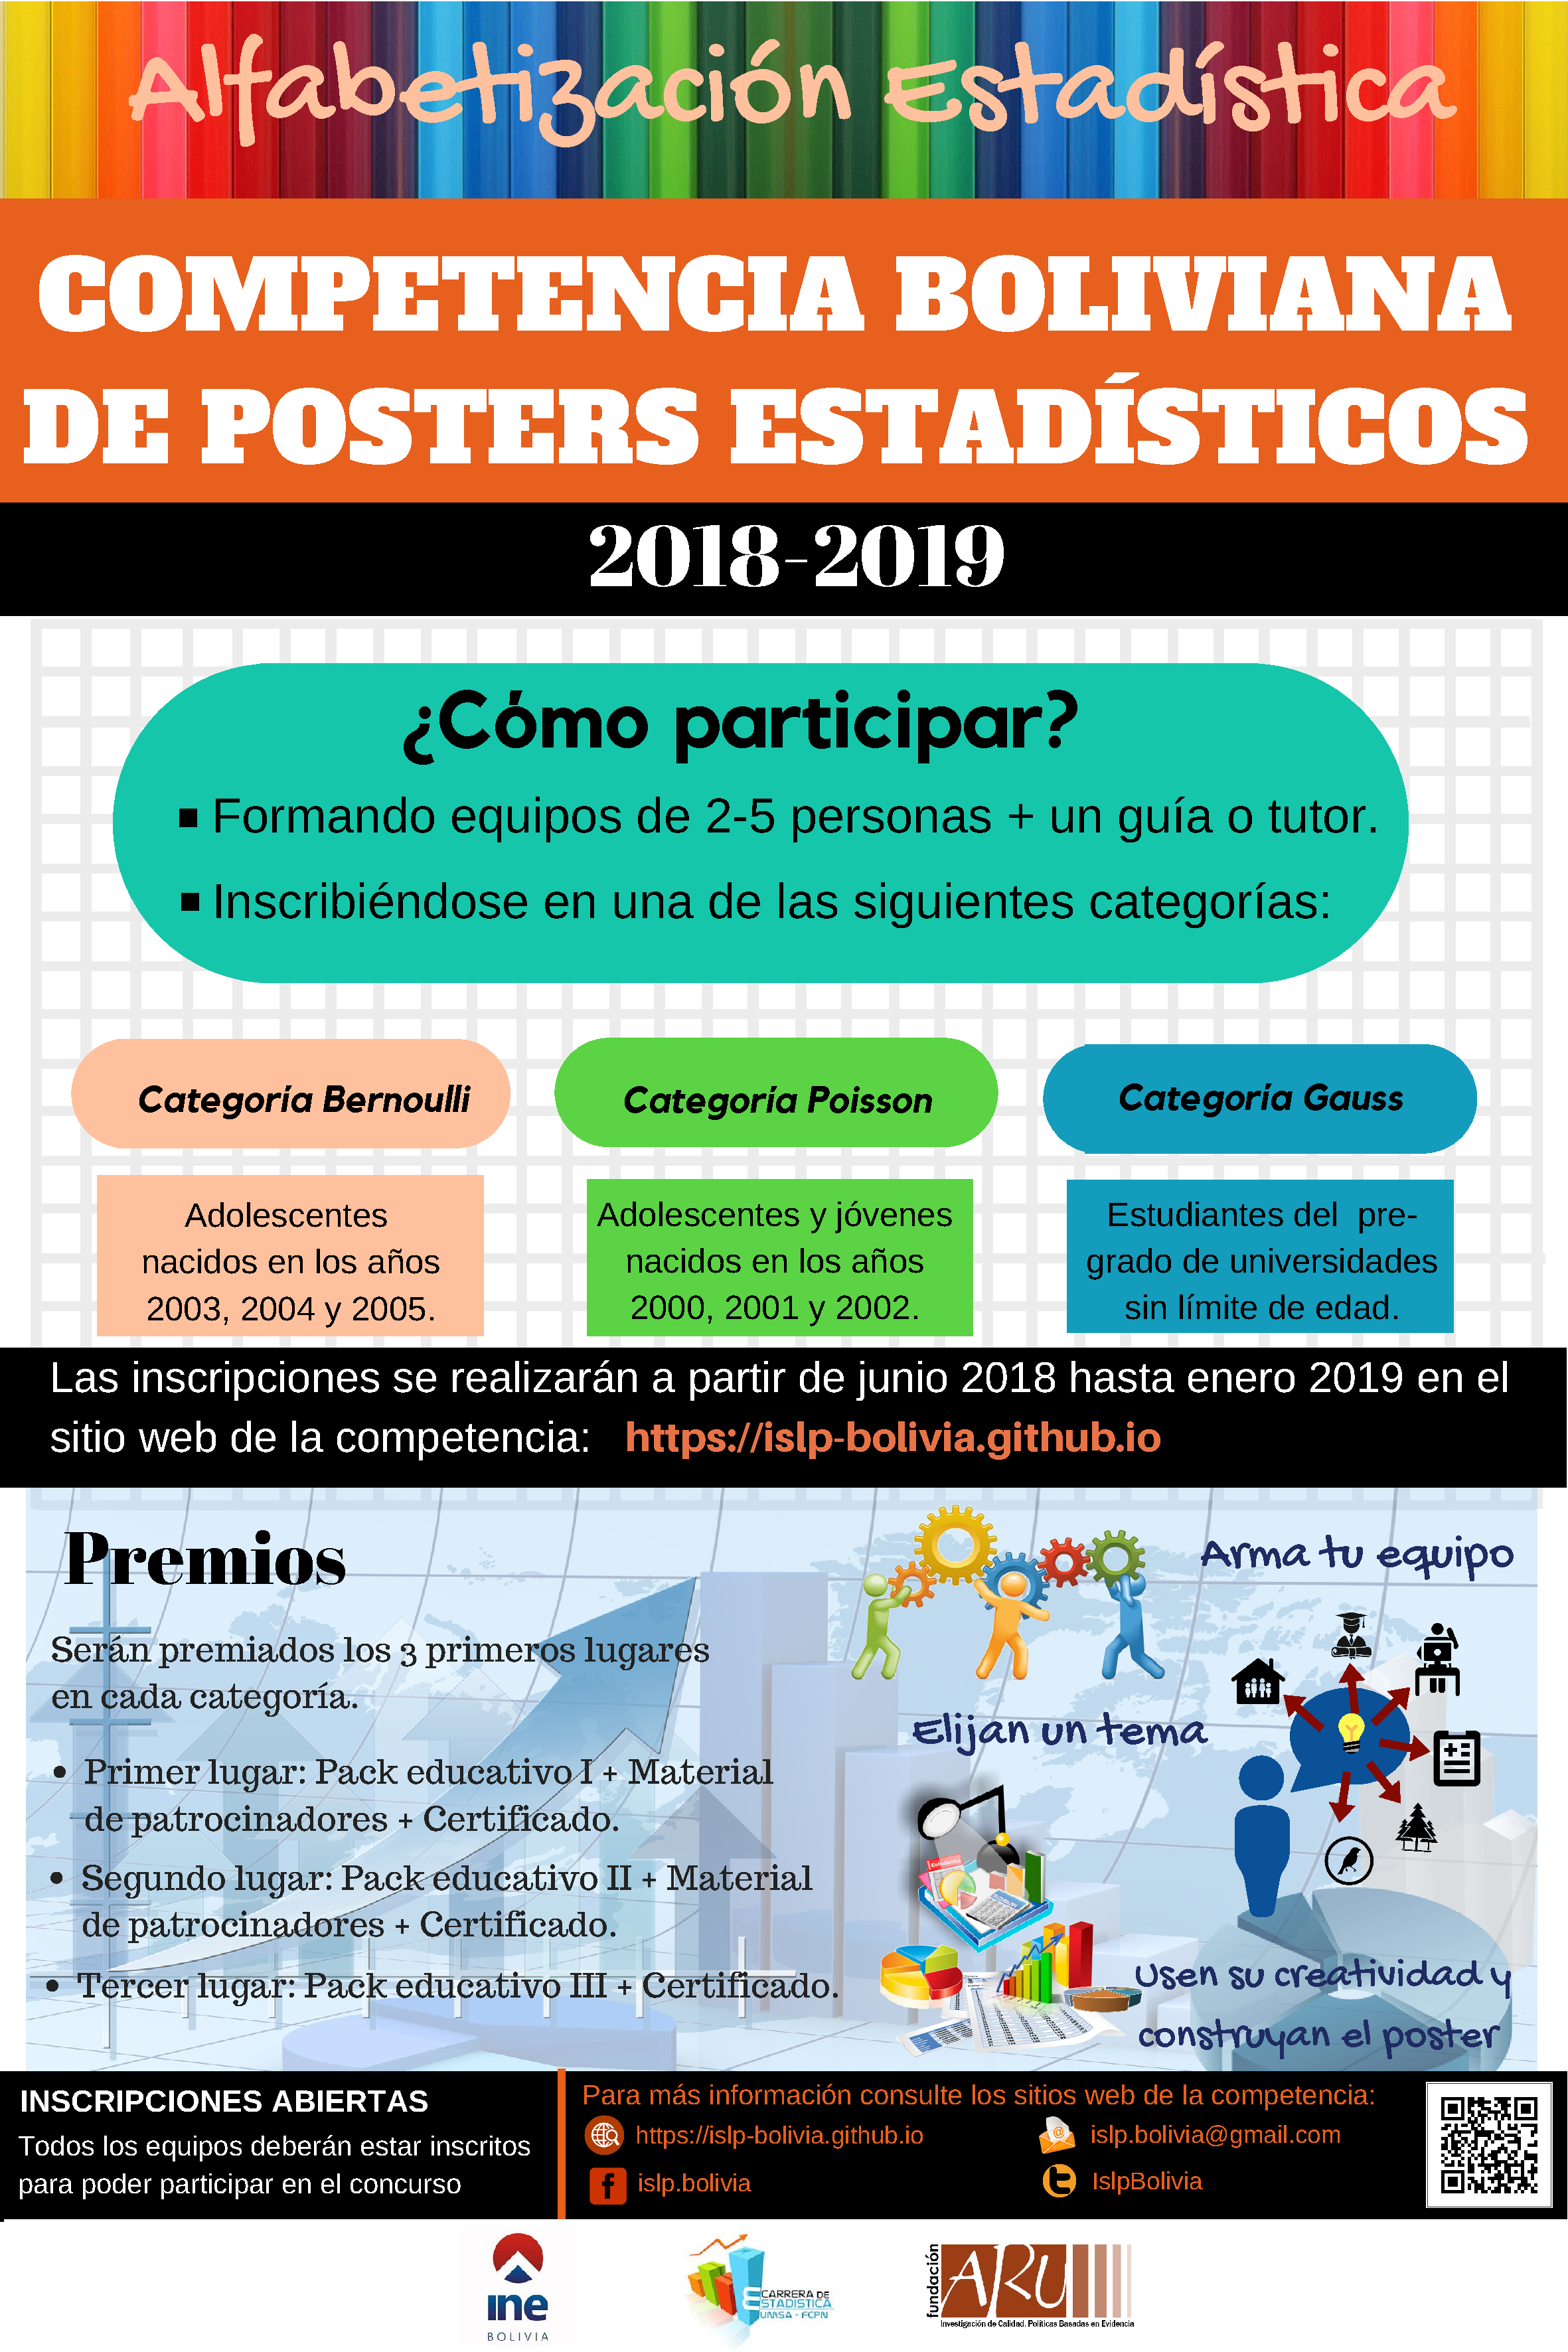
\includepdf[pages=-]{poster}

%\newpage

%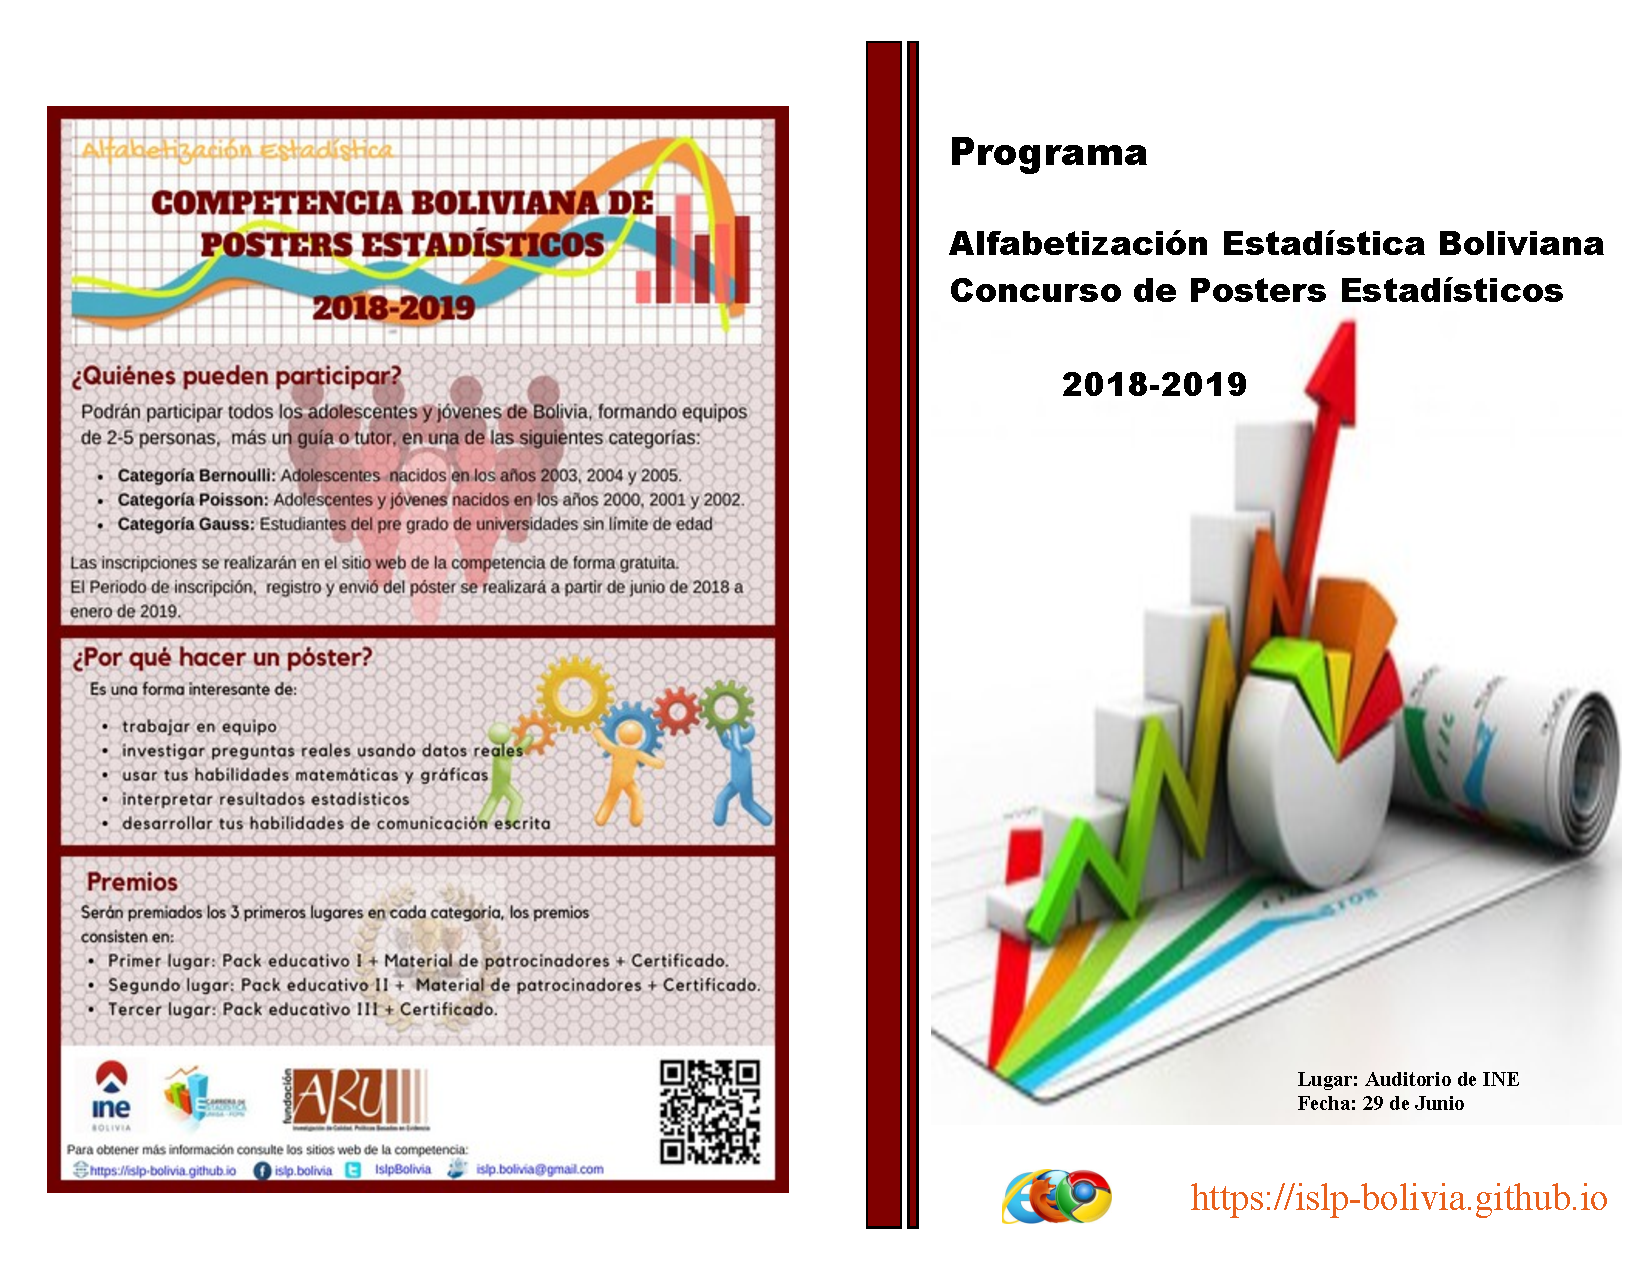
\includepdf[pages=-]{Programa}
\end{document}